% chapter2.tex
\chapter{理论基础与相关技术}
\label{chap:theory}

\section{公式排版示例}
本节展示数学公式的排版方法。行内公式可以直接使用 \verb|$...$| 包裹，例如著名的质能方程 $E = mc^2$。如果是独立的居中公式，应使用 \verb|equation| 环境，如式\ref{eq:emc}所示：

\begin{equation}
    E = mc^2
    \label{eq:emc}
\end{equation}

对于复杂的多行公式，可以使用 \verb|aligned| 或 \verb|gather| 环境：

\begin{equation}
    \begin{aligned}
        \min_{\theta} \quad & \mathcal{L}(\theta) = \frac{1}{N} \sum_{i=1}^{N} L(f_\theta(x_i), y_i) \\
        \text{s.t.} \quad & ||\theta||_2 \leq C
    \end{aligned}
\end{equation}

\section{表格排版示例}
本节展示如何在论文中排版规范的三线表。根据排版规范，表格的表题应位于表格的**正上方**居中，字号为五号黑体。在 LaTeX 中，我们通常使用 \verb|booktabs| 宏包提供的 \verb|\toprule|、\verb|\midrule| 和 \verb|\bottomrule| 来绘制三线表。如表\ref{tab:sample_table}所示：

\begin{table}[htbp]
    \centering
    \caption{示例三线表排版说明}
    \label{tab:sample_table}
    \begin{tabular}{llcc}
        \toprule
        \textbf{序号} & \textbf{测试项目} & \textbf{准确率 (\%)} & \textbf{延迟 (ms)} \\
        \midrule
        1 & 基础模型测试 & 92.5 & 120 \\
        2 & 改进模型A测试 & 95.2 & 135 \\
        3 & 改进模型B测试 & \textbf{96.8} & 110 \\
        \bottomrule
    \end{tabular}
\end{table}

\section{图片排版示例}
本节展示图片的插入方法。根据规范，图题应位于图片的**正下方**居中，字号为小五号黑体。所有图片文件请放置在根目录下的 \verb|figures/| 文件夹中。

这里我们插入一张格式检测的报告截图作为示例，如图\ref{fig:sample_figure}所示。

\begin{figure}[htbp]
    \centering
    % 宽度可以设置为页面宽度的比例，如 0.8\textwidth
    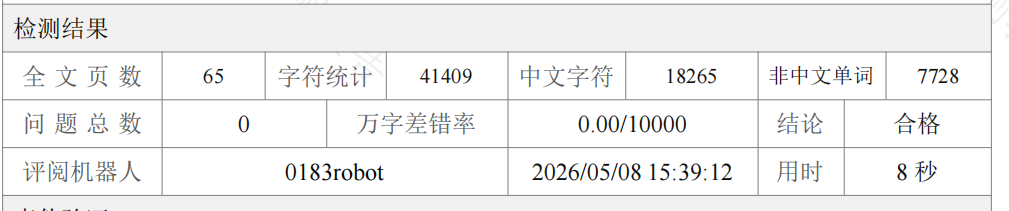
\includegraphics[width=0.8\textwidth]{assets/格式检测结果.png}
    \caption{格式检测系统结果示例图}
    \label{fig:sample_figure}
\end{figure}

如果需要并排插入多张子图，可以利用 \verb|subcaption| 宏包提供的 \verb|subfigure| 环境来实现。

\section{参考文献引用示例}
本节展示参考文献的交叉引用方法。本模板已经集成了基于 \verb|biblatex| 的国标 GB/T 7714-2015 样式宏包，所有的参考文献信息均存储在 \verb|references.bib| 文件中。

\begin{itemize}
    \item \textbf{上标引用}：这是最常用的引用方式，如“在深度学习领域，Hinton等人的研究\cite{hinton2012deep}奠定了基础”。
    \item \textbf{多重引用}：可以同时引用多篇文献，如“语音分离技术经历了快速的发展\cite{luo2019conv, lu2024music}”。
    \item \textbf{作为句法成分（非上标）}：如果文献编号作为句子的一部分，应使用 \verb|\parencite|，如“详细的推导过程可参考文献 \parencite{wang2006computational} 的第三章”。
\end{itemize}

请注意，你只需要在 \verb|references.bib| 中按照 BibTeX 格式填好条目信息，并在文中使用 \verb|\cite|，文末的参考文献列表会自动生成，并且悬挂缩进等格式均符合学校的最新排版要求。
